% Compile with:  pdflatex exposure_design_diagram.tex
\documentclass[tikz,border=12pt]{standalone}
\usepackage{tikz}
\usetikzlibrary{decorations.pathreplacing, calligraphy, positioning, fit}
\usepackage{amsmath}
\begin{document}
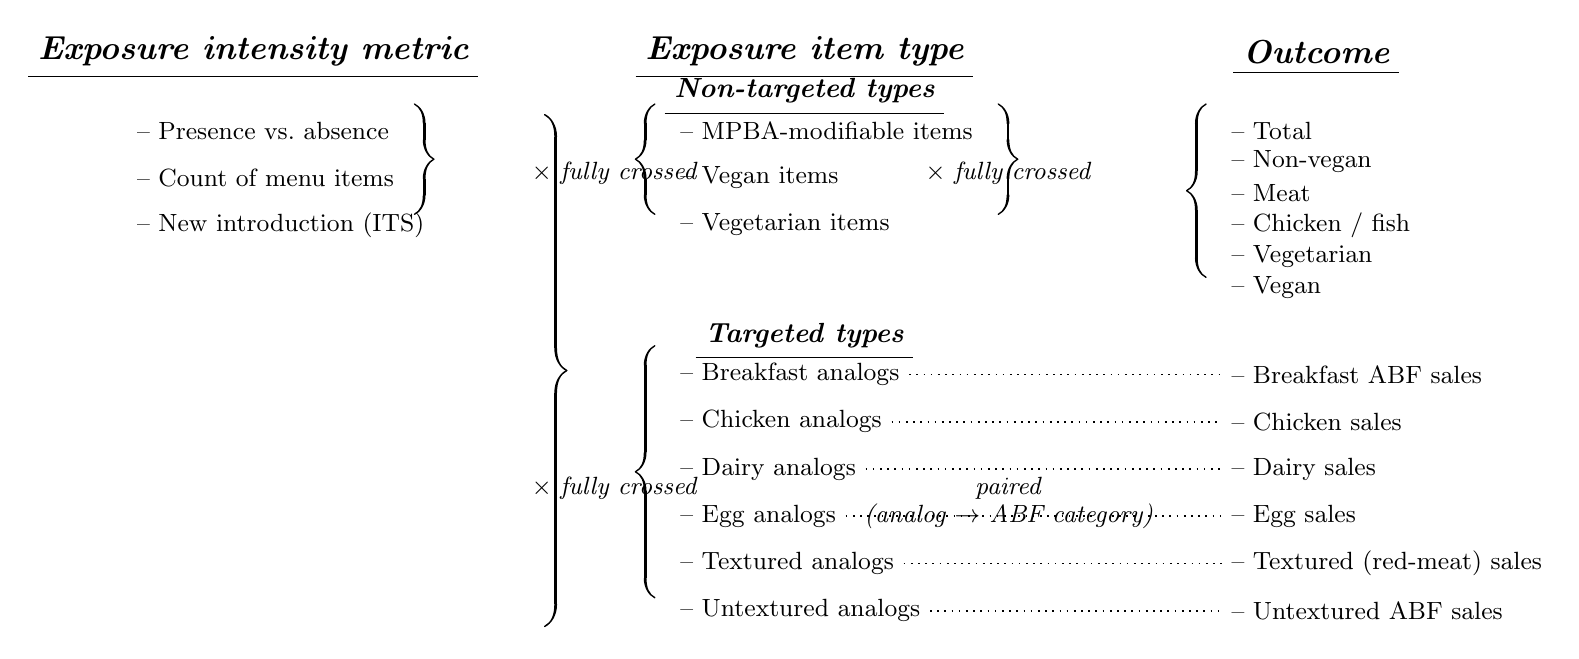
\begin{tikzpicture}[
    font=\small,
    node distance=4pt,
    item/.style={anchor=west},
    header/.style={font=\itshape\bfseries\large}
]

% ── Column headers ──────────────────────────────────────────
\node[header] (h1) at (0,7)   {Exposure intensity metric};
\node[header] (h2) at (7,7)   {Exposure item type};
\node[header] (h3) at (13.5,7){Outcome};
\draw[line width=0.4pt] (h1.south west) -- (h1.south east);
\draw[line width=0.4pt] (h2.south west) -- (h2.south east);
\draw[line width=0.4pt] (h3.south west) -- (h3.south east);

% ── Col 1: intensity ───────────────────────────────────────
\node[item] (i1) at (-1.6, 6.0) {-- Presence vs.\ absence};
\node[item] (i2) at (-1.6, 5.4) {-- Count of menu items};
\node[item] (i3) at (-1.6, 4.8) {-- New introduction (ITS)};

% ── Col 2 upper: non-targeted types ───────────────────────
\node[font=\itshape\bfseries] (nth) at (7, 6.5) {Non-targeted types};
\draw[line width=0.3pt] (nth.south west) -- (nth.south east);
\node[item] (n1) at (5.3, 6.0) {-- MPBA-modifiable items};
\node[item] (n2) at (5.3, 5.4) {-- Vegan items};
\node[item] (n3) at (5.3, 4.8) {-- Vegetarian items};

% ── Col 2 lower: targeted types ───────────────────────────
\node[font=\itshape\bfseries] (th) at (7, 3.4) {Targeted types};
\draw[line width=0.3pt] (th.south west) -- (th.south east);
\node[item] (t1) at (5.3, 2.9) {-- Breakfast analogs};
\node[item] (t2) at (5.3, 2.3) {-- Chicken analogs};
\node[item] (t3) at (5.3, 1.7) {-- Dairy analogs};
\node[item] (t4) at (5.3, 1.1) {-- Egg analogs};
\node[item] (t5) at (5.3, 0.5) {-- Textured analogs};
\node[item] (t6) at (5.3,-0.1) {-- Untextured analogs};

% ── Col 3 upper: outcomes ─────────────────────────────────
\node[item] (o1) at (12.3, 6.0) {-- Total};
\node[item] (o2) at (12.3, 5.6) {-- Non-vegan};
\node[item] (o3) at (12.3, 5.2) {-- Meat};
\node[item] (o4) at (12.3, 4.8) {-- Chicken / fish};
\node[item] (o5) at (12.3, 4.4) {-- Vegetarian};
\node[item] (o6) at (12.3, 4.0) {-- Vegan};

% ── Col 3 lower: paired outcomes ──────────────────────────
\node[item] (p1) at (12.3, 2.9) {-- Breakfast ABF sales};
\node[item] (p2) at (12.3, 2.3) {-- Chicken sales};
\node[item] (p3) at (12.3, 1.7) {-- Dairy sales};
\node[item] (p4) at (12.3, 1.1) {-- Egg sales};
\node[item] (p5) at (12.3, 0.5) {-- Textured (red-meat) sales};
\node[item] (p6) at (12.3,-0.1) {-- Untextured ABF sales};

% ── Pair connectors (dotted) ──────────────────────────────
\foreach \a/\b in {t1/p1, t2/p2, t3/p3, t4/p4, t5/p5, t6/p6}
    \draw[dotted, line width=0.6pt] (\a.east) -- (\b.west);

% ── Curly braces around each group ────────────────────────
\draw[decorate, decoration={calligraphic brace, amplitude=7pt}, line width=1pt]
    (i1.north east) ++(0.2,0.1) -- ++(0,-1.4);                % intensity col
\draw[decorate, decoration={calligraphic brace, mirror, amplitude=7pt}, line width=1pt]
    (n1.north west) ++(-0.2,0.1) -- ++(0,-1.4);                % non-targeted left
\draw[decorate, decoration={calligraphic brace, amplitude=7pt}, line width=1pt]
    (n1.north east) ++(0.2,0.1) -- ++(0,-1.4);                 % non-targeted right
\draw[decorate, decoration={calligraphic brace, mirror, amplitude=7pt}, line width=1pt]
    (t1.north west) ++(-0.2,0.1) -- ++(0,-3.2);                % targeted left
\draw[decorate, decoration={calligraphic brace, mirror, amplitude=7pt}, line width=1pt]
    (o1.north west) ++(-0.2,0.1) -- ++(0,-2.2);                % outcomes left

% Big brace to the right of intensity, covering both item-type groups
\draw[decorate, decoration={calligraphic brace, amplitude=8pt}, line width=1pt]
    (3.7, 6.2) -- (3.7, -0.3);

% ── Cross labels ──────────────────────────────────────────
\node at (4.6, 5.45) {$\times$ \textit{\small fully crossed}};
\node at (9.6, 5.45) {$\times$ \textit{\small fully crossed}};
\node at (4.6, 1.45) {$\times$ \textit{\small fully crossed}};
\node at (9.6, 1.45) {\textit{\small paired}};
\node at (9.6, 1.10) {\textit{\small (analog $\to$ ABF category)}};

\end{tikzpicture}
\end{document}
